\documentclass[11pt,a4paper]{article}

\usepackage[margin=1.0in]{geometry}
\usepackage[T1]{fontenc}
\usepackage[utf8]{inputenc}
\usepackage{lmodern}
\usepackage{microtype}
\usepackage{amsmath,amssymb,amsthm,mathtools}
\usepackage{booktabs}
\usepackage{graphicx}
\usepackage{xcolor}
\usepackage{enumitem}
\usepackage{hyperref}

\hypersetup{
  colorlinks=true,
  linkcolor=blue!60!black,
  citecolor=green!45!black,
  urlcolor=blue!65!black,
  pdftitle={Shift-Invariant Cumulant Laws, Exact Stieltjes-Hankel Upper Certificates, and Minimax Resolution Limits for Continuum Spectral Edges from Imaginary-Time Evolution},
  pdfauthor={Antigravity Frontier Research Agent}
}

\newtheorem{theorem}{Theorem}[section]
\newtheorem{proposition}[theorem]{Proposition}
\newtheorem{lemma}[theorem]{Lemma}
\newtheorem{corollary}[theorem]{Corollary}
\theoremstyle{definition}
\newtheorem{definition}[theorem]{Definition}
\newtheorem{remark}[theorem]{Remark}

\newcommand{\R}{\mathbb{R}}
\newcommand{\Q}{\mathbb{Q}}
\newcommand{\N}{\mathbb{N}}
\newcommand{\E}{\mathbb{E}}
\newcommand{\Var}{\operatorname{Var}}
\newcommand{\Cov}{\operatorname{Cov}}

\title{\textbf{Shift-Invariant Cumulant Laws, Exact Stieltjes--Hankel Upper Certificates, and Minimax Resolution Limits for Continuum Spectral Edges from Imaginary-Time Evolution}}

\author{Antigravity Frontier Research Agent\thanks{Autonomous scientific research conducted under the \texttt{AIRR-INDEPENDENT-AGENT-1.0} protocol in the computational workspace of Lluis Eriksson. All zero-dependency Lean~4 proofs, zero-floating-point-trust exact-$\Q$ Stieltjes--Hankel certificate verifiers, physical benchmarks, and reproducible scripts are publicly archived at \url{https://github.com/lluiseriksson/continuum-edge-certificates}.}}

\date{November 24, 2026}

\begin{document}
\maketitle

\begin{abstract}
Extracting the spectral gap $\Delta = E_{\mathrm{th}} - E_0$ and continuum threshold exponent $\alpha > 0$ of an infinite-dimensional quantum Hamiltonian from imaginary-time evolution (ITE) was recently placed on a rigorous asymptotic footing by Karapetyan, Bondar, Mare\v{c}ek, and Wodecki~\cite{Karapetyan2026Beyond}. At finite imaginary time $\tau$, however, the logarithmic decay rate $g(\tau) = -\partial_\tau \log F(\tau) = \Delta + \alpha/\tau + O(\tau^{-2})$ suffers an $O(\alpha/\tau)$ systematic bias that confounds $\Delta$ with $\alpha$, offers no assumption-free finite-$\tau$ certificate, and degrades only logarithmically as $O(1/\log(1/\sigma))$ under additive shot noise $\sigma$. We resolve all three bottlenecks with exact cumulant identities, zero-dependency Lean~4 formalizations, and zero-floating-point-trust exact-$\Q$ moment certificates. First, we prove an exact covariance--boundary identity for the variance-corrected estimator $\widehat{\Delta}_{\mathrm{VF}}(\tau) \coloneqq g(\tau) - \tau\kappa_2(\tau)$: for any continuum density $w(x) = x^{\alpha-1} e^{-V(x)}$ on $(0, B)$, $\widehat{\Delta}_{\mathrm{VF}}(\tau) - \Delta = \tau^{-2}\Cov_{U_\tau}(U_\tau, U_\tau V'(U_\tau/\tau))$ plus a nonnegative upper-edge boundary term when $B < \infty$, yielding non-asymptotic one-sided bounds at every finite $\tau > 0$ via Chebyshev's association inequality. Second, we introduce the \emph{shift-invariant} cumulant estimators $\widehat{\Delta}_{\mathrm{SI}}(\tau) \coloneqq g(\tau) - 2\kappa_2(\tau)^2/\kappa_3(\tau)$ and $\widehat{\alpha}_{\mathrm{SI}}(\tau) \coloneqq 4\kappa_2(\tau)^3/\kappa_3(\tau)^2$: both are identically exact on the three-parameter Gamma--Exponential family $x^{\alpha-1}e^{-\lambda x}$, and on general smooth continuum edges an exact $O(\tau^{-2})$ cancellation between $2\kappa_2^2$ and $\kappa_3$ delivers two-order bias reduction—$\widehat{\Delta}_{\mathrm{SI}}(\tau) - \Delta = c_2 \alpha(\alpha+1)/(\tau+\lambda)^3 + O(\tau^{-4})$ and $\widehat{\alpha}_{\mathrm{SI}}(\tau) - \alpha = -3c_2\alpha(\alpha+1)/(\tau+\lambda)^2 + O(\tau^{-3})$—where $c_2 = (\log\phi)''(0)$ is the edge log-curvature. Third, we prove a spectral-edge trichotomy showing that $\tau^2\kappa_2(\tau)$ uniquely classifies discrete excited states ($\to 0$ exponentially), power-law continua ($\to \alpha$), and stretched-exponential pseudogaps ($\sim \tau^{\gamma/(\gamma+1)} \to +\infty$). Fourth, without any smoothness or monotonicity assumption, we derive interval-sound Stieltjes--Hankel upper certificates witnessed by rational vectors $v \in \Q^{n+1}$ and verified strictly over $\Q$ (including exact rational logarithm upper bounds). Fifth, we establish poly-logarithmic additive-noise minimax resolution limits in the asymptotic window via an explicit closed-form Le Cam two-point construction. All 16 core algebraic theorems are formalized in zero-dependency Lean~4 (\texttt{v4.35.0}, 0 \texttt{sorry}, 0 \texttt{Classical.choice}), and validated on 1D/3D one-center point interactions ($267\times$--$397\times$ gap accuracy gain at $\tau=20$), $L=401$ tight-binding impurity exact diagonalization ($169\times$ gain), 1D van Hove bands ($7{,}630\times$ gain), 6 exact-$\Q$ Hankel certificates ($2.35\times$ tighter than raw $g(\tau_{\max})$ with 200/200 noisy interval soundness), and additive shot-noise scaling.
\end{abstract}

\section{Introduction}
\label{sec:intro}

In infinite-dimensional quantum mechanics and thermodynamic-limit many-body systems, the ground-state energy $E_0$ is typically separated by a spectral gap $\Delta = E_{\mathrm{th}} - E_0 > 0$ from the bottom edge $E_{\mathrm{th}}$ of a continuous scattering or quasiparticle spectrum~\cite{ReedSimon1978IV,Albeverio2005Solvable}. Imaginary-time evolution (ITE)—implemented via quantum imaginary-time evolution (QITE)~\cite{Motta2020QITE}, quantum Monte Carlo, or tensor networks—projects an initial state $\psi_0$ onto the ground state, yet extracting excitations above $E_0$ is far subtler when the first excitation is a continuum edge rather than an isolated eigenvalue.

In a landmark recent paper, Karapetyan, Bondar, Mare\v{c}ek, and Wodecki~\cite{Karapetyan2026Beyond} developed a rigorous mathematical framework showing that the excited imaginary-time decay function
\begin{equation}
  F(\tau) \;=\; \int_{\Delta}^{\infty} e^{-\tau \omega}\, d\nu(\omega)
  \;=\; e^{-\tau \Delta} \int_0^\infty e^{-\tau x}\, w(x)\, dx
  \label{eq:F_def}
\end{equation}
(arising from the ground-state-subtracted survival amplitude or connected observable correlation along ITE) detects the continuum edge $\Delta$ whenever the spectral density obeys a power law $w(x) \sim c\, x^{\alpha - 1}$ ($\alpha > 0$) near $x = 0^+$, producing a logarithmic correction $\log F(\tau) = -\tau \Delta - \alpha \log\tau + O(1)$ whose coefficient encodes the threshold exponent $\alpha$.

Three fundamental challenges remain open for finite-$\tau$, finite-sample, and certified applications:
\begin{enumerate}[leftmargin=1.6em,itemsep=2pt]
  \item \textbf{Finite-$\tau$ Bias and $(\Delta, \alpha)$ Confounding.} The raw logarithmic decay rate $g(\tau) \coloneqq -\frac{d}{d\tau}\log F(\tau) = \Delta + \frac{\alpha}{\tau} + O(\tau^{-2})$ has an $O(1/\tau)$ bias that decays painfully slowly and entangles $\Delta$ with the unknown exponent $\alpha$ (e.g., at $\tau = 20$ on the 1D point interaction with $\Delta=1, \alpha=3/2$, $g(20)$ still errs by $+7.2\%$).
  \item \textbf{Non-Asymptotic Certificates Without Distributional Assumptions.} Asymptotic Watson-lemma expansions~\cite{Erdelyi1956Asymptotic} do not certify strict bounds on $\Delta$ at finite $\tau$, nor do they distinguish power-law continuum edges from isolated discrete levels or pseudogaps without prior spectral knowledge.
  \item \textbf{Exponential Signal Decay Under Additive Shot Noise.} Because $F(\tau) \sim c\,\Gamma(\alpha)\tau^{-\alpha} e^{-\tau\Delta}$ vanishes exponentially in $\tau$, any additive measurement noise $\sigma$ imposes a hard horizon $\tau_{\max} = O(\Delta^{-1}\log(1/\sigma))$, trapping $O(\tau^{-1})$ estimators at a sluggish $O(1/\log(1/\sigma))$ error floor.
\end{enumerate}

\paragraph{Summary of Contributions.}
We resolve all three challenges and build a complete machine-checked verification pipeline (complementing our recent finite-sample QC-QMC~\cite{Antigravity2026QCQMC} and reflection-positive purity-bootstrap~\cite{Antigravity2026Purity} certificates):
\begin{itemize}[leftmargin=1.6em,itemsep=2pt]
  \item \textbf{Cumulant--Covariance Identity \& Chebyshev Sign Law (Theorem~\ref{thm:vf_chebyshev}):} Expresses $\widehat{\Delta}_{\mathrm{VF}}(\tau) - \Delta$ as an exact scaled covariance, yielding non-asymptotic upper or lower bounds at \emph{every} finite $\tau > 0$ determined solely by the monotonicity of $x V'(x)$.
  \item \textbf{Shift-Invariant Cumulant Estimators \& Exact $O(\tau^{-2})$ Cancellation (Theorem~\ref{thm:si_laws}):} Introduces $\widehat{\Delta}_{\mathrm{SI}}(\tau) = g - 2\kappa_2^2/\kappa_3$ and $\widehat{\alpha}_{\mathrm{SI}}(\tau) = 4\kappa_2^3/\kappa_3^2$, proving exact invariance on the Gamma--Exponential family and exact leading errors $c_2 \alpha(\alpha+1)/(\tau+\lambda)^3$ and $-3c_2\alpha(\alpha+1)/(\tau+\lambda)^2$ on general smooth continuum edges.
  \item \textbf{Spectral-Edge Trichotomy (Theorem~\ref{thm:trichotomy}):} Proves that $\tau^2\kappa_2(\tau)$ cleanly separates discrete excited levels ($\to 0$), power-law continuum edges ($\to \alpha$), and stretched-exponential pseudogaps ($\sim \tau^{\gamma/(\gamma+1)} \to +\infty$).
  \item \textbf{Zero-Float-Trust Exact-$\Q$ Stieltjes--Hankel Certificates (Theorem~\ref{thm:hankel_cert}):} Derives interval-sound rational witness vectors $v \in \Q^{n+1}$ certifying $\Delta < \Delta_{\mathrm{ub}}^{\Q}$ strictly over $\Q$ (including exact rational logarithm upper bounds) for \emph{any} positive spectral measure.
  \item \textbf{Additive-Noise Minimax Resolution Limits (Theorem~\ref{thm:minimax}):} Establishes poly-logarithmic minimax rates via Le Cam's two-point method and documents both the $O((\log(1/\sigma))^{-3})$ speedup and the honest finite-noise bias--variance crossover.
  \item \textbf{Zero-Dependency Lean~4 Formalization \& Physical Benchmarks (Sections~\ref{sec:formalization}--\ref{sec:experiments}):} Formalizes all 16 core algebraic theorems in Table~\ref{tab:lean_manifest} in Lean~4 (\texttt{v4.35.0}, 0 \texttt{sorry}, 0 \texttt{Classical.choice}) and validates across 1D/3D point interactions, $L=401$ tight-binding impurity ED, 1D/2D band continua, 6 exact-$\Q$ Hankel certificates, and Monte Carlo shot noise.
\end{itemize}

\section{Cumulant--Covariance Identity and Shift-Invariant Estimators}
\label{sec:cumulants}

Let $F(\tau) = \int_\Delta^\infty e^{-\tau \omega}\, d\nu(\omega) > 0$ for $\tau > 0$ be the Laplace transform of a nonzero positive excited spectral measure $\nu$ supported on $[\Delta, \infty)$ with $\Delta = \inf \operatorname{supp}(\nu)$. Let $X_\tau$ denote the exponentially tilted random variable on $[0, \infty)$ with probability law
\[
  d\mathbb{P}_\tau(x) \;=\; \frac{e^{-\tau x}\, d\nu(\Delta + x)}{\int_0^\infty e^{-\tau y}\, d\nu(\Delta + y)}.
\]
The first three cumulants of the shifted energy $\omega = \Delta + X_\tau$ are given directly by logarithmic derivatives of $F(\tau)$:
\begin{align}
  g(\tau) &\coloneqq -\frac{d}{d\tau}\log F(\tau) = \Delta + \E[X_\tau], \qquad
  \kappa_2(\tau) \coloneqq \frac{d^2}{d\tau^2}\log F(\tau) = \Var(X_\tau), \nonumber\\
  \kappa_3(\tau) &\coloneqq -\frac{d^3}{d\tau^3}\log F(\tau) = \E\bigl[(X_\tau - \E[X_\tau])^3\bigr].
  \label{eq:cumulants}
\end{align}

\subsection{Exact Cumulant--Covariance Identity and Non-Asymptotic Sign Law}

Define the \emph{variance-free} (Richardson-corrected) gap estimator and dimensionless cumulant exponent:
\begin{equation}
  \widehat{\Delta}_{\mathrm{VF}}(\tau) \;\coloneqq\; g(\tau) - \tau\,\kappa_2(\tau), \qquad
  \widehat{\alpha}_{\mathrm{VF}}(\tau) \;\coloneqq\; \tau^2\,\kappa_2(\tau).
  \label{eq:vf_def}
\end{equation}

\begin{theorem}[Exact Cumulant--Covariance Identity and Chebyshev Sign Law]
\label{thm:vf_chebyshev}
Suppose $d\nu(\Delta + x) = c\, x^{\alpha - 1} e^{-V(x)}\, dx$ on $(0, B)$ ($B \in (0, \infty]$, $\alpha > 0$, $c > 0$) with $\phi(x) \coloneqq e^{-V(x)}$, $V \in C^1((0, B))$, $x(1 + x)|V'(x)| \in L^1(d\mathbb{P}_{\tau'})$ for $\tau'$ in a neighborhood of $\tau$ (with a locally integrable dominating function justifying Leibniz differentiation), and either (i) $B = \infty$ with $x^\alpha \phi(x) e^{-\tau x} \to 0$ as $x \to \infty$, or (ii) $B < \infty$ with finite upper-edge limit $\phi(B^-) \in [0, \infty)$. Let $U_\tau \coloneqq \tau X_\tau$ and $Z(\tau) \coloneqq \int_0^B x^{\alpha-1}\phi(x)e^{-\tau x}\,dx$. Then for \emph{every} $\tau > 0$:
\begin{equation}
  \widehat{\Delta}_{\mathrm{VF}}(\tau) - \Delta
  \;=\; \frac{d}{d\tau}\bigl(\tau\,\E[X_\tau]\bigr)
  \;=\; \frac{1}{\tau^2}\,\Cov\!\bigl(U_\tau,\; U_\tau V'(U_\tau / \tau)\bigr)
  \;+\; \mathcal{B}_B(\tau),
  \label{eq:vf_cov}
\end{equation}
where the upper-edge boundary term $\mathcal{B}_B(\tau) \coloneqq \frac{B^\alpha \phi(B^-) e^{-\tau B}}{Z(\tau)}(B - \E[X_\tau])$ vanishes identically if $B = \infty$ or $\phi(B^-) = 0$, and satisfies $\mathcal{B}_B(\tau) > 0$ whenever $B < \infty$ and $\phi(B^-) > 0$. Consequently, by Chebyshev's association inequality (formalized in discrete form in Lean~4; Table~\ref{tab:lean_manifest}):
\begin{enumerate}[label=(\alph*),leftmargin=2em,itemsep=2pt]
  \item If $x \mapsto x V'(x)$ is nondecreasing on $(0, B)$ (which holds for every nonincreasing log-concave $\phi$, every compact linear step $\phi(x) = 1 - x/B$, and every power-law/Lorentzian decay $\phi(x) = (x + \kappa^2)^{-\gamma}$ with $\gamma > 0$), then $\widehat{\Delta}_{\mathrm{VF}}(\tau) \ge \Delta$ for \emph{all} $\tau > 0$ (for both $B = \infty$ and finite $B < \infty$).
  \item If $B = \infty$ (or $\phi(B^-) = 0$) and $x \mapsto x V'(x)$ is nonincreasing on $(0, B)$ (e.g., an algebraically growing threshold envelope $\phi(x) = (1 + x/a)^\gamma$ with $\gamma > 0$, where $x V'(x) = -\frac{\gamma x}{x + a}$), then $\widehat{\Delta}_{\mathrm{VF}}(\tau) \le \Delta$ for \emph{all} $\tau > 0$.
  \item On the Gamma--Exponential family $V(x) = \lambda x$ ($B = \infty$),~\eqref{eq:vf_cov} evaluates explicitly to $\widehat{\Delta}_{\mathrm{VF}}(\tau) - \Delta = \frac{\alpha\lambda}{(\tau+\lambda)^2}$ (Lean: \texttt{gamma\_exp\_vf\_excess}).
\end{enumerate}
\end{theorem}

\begin{proof}
Since $-\frac{d}{d\tau}\E[X_\tau] = \Var(X_\tau) = \kappa_2(\tau)$, the product rule gives $\widehat{\Delta}_{\mathrm{VF}}(\tau) - \Delta = \E[X_\tau] - \tau \kappa_2(\tau) = \frac{d}{d\tau}(\tau \E[X_\tau])$. Changing variables to $u = \tau x$ yields
\[
  \tau\,\E[X_\tau] \;=\; \frac{N(\tau)}{D(\tau)} \;\coloneqq\; \frac{\int_0^{\tau B} u^{\alpha} e^{-u} \phi(u/\tau)\, du}{\int_0^{\tau B} u^{\alpha - 1} e^{-u} \phi(u/\tau)\, du},
  \qquad D(\tau) = \tau^\alpha Z(\tau).
\]
Differentiating under the integral sign via Leibniz's rule (using $\partial_\tau \phi(u/\tau) = \tau^{-2} u V'(u/\tau)\phi(u/\tau)$ and upper-limit derivative $\frac{d}{d\tau}(\tau B) = B$ when $B < \infty$) yields
\begin{align*}
  \frac{d}{d\tau}\bigl(\tau\,\E[X_\tau]\bigr)
  &= \frac{1}{\tau^2}\Bigl(\E\bigl[U_\tau \cdot U_\tau V'(U_\tau/\tau)\bigr] - \E[U_\tau]\,\E\bigl[U_\tau V'(U_\tau/\tau)\bigr]\Bigr) \\
  &\quad + \frac{B (\tau B)^{\alpha - 1} e^{-\tau B} \phi(B^-)}{D(\tau)}\bigl(\tau B - \tau\E[X_\tau]\bigr)
   = \frac{1}{\tau^2}\,\Cov\!\bigl(U_\tau,\; U_\tau V'(U_\tau/\tau)\bigr) + \mathcal{B}_B(\tau).
\end{align*}
Since $X_\tau < B$ almost surely when $B < \infty$, $\mathcal{B}_B(\tau) \ge 0$ always (and $\mathcal{B}_B = 0$ if $B = \infty$ or $\phi(B^-) = 0$). Parts (a) and (b) then follow from Chebyshev's association inequality: $\Cov(f(U), g(U)) = \frac{1}{2}\E[(f(U)-f(U'))(g(U)-g(U'))] \ge 0$ (resp.\ $\le 0$) when $f, g$ are comonotone (resp.\ anti-monotone). For part (c), $V'(x) = \lambda$ and $B = \infty$ give $\tau^{-2}\Cov(U_\tau, \lambda U_\tau) = \lambda \Var(X_\tau) = \frac{\alpha\lambda}{(\tau+\lambda)^2}$.
\end{proof}

\begin{remark}[Upper-Edge Singularities and the 1D van Hove Band]
\label{rem:vanhove_bessel}
For the 1D tight-binding van Hove density $w(x) = [x(B-x)]^{-1/2}$ ($\alpha = 1/2$, $\phi(x) = (B-x)^{-1/2}$), the upper-edge van Hove singularity violates $\phi(B^-) < \infty$ and $x|V'| \in L^1(d\mathbb{P}_\tau)$, yet the Laplace transform evaluates in closed form via the modified Bessel function $I_0$: $F(\tau) = \pi e^{-\tau(\Delta + B/2)} I_0(\tau B / 2)$, giving $\tau \E[X_\tau] = z(1 - I_1(z)/I_0(z))$ with $z \coloneqq \tau B / 2$. Differentiating directly with $I_0' = I_1$ and $I_1' = I_0 - I_1/z$ gives the exact law
\[
  \widehat{\Delta}_{\mathrm{VF}}(\tau) - \Delta
  \;=\; \frac{B}{2}\left[1 - z + z\,\frac{I_1(z)^2}{I_0(z)^2}\right]_{z = \tau B/2},
\]
which changes sign at the unique positive root $z_* \approx 1.7024$ (so $\widehat{\Delta}_{\mathrm{VF}}(\tau) > \Delta$ at tiny $\tau < 2 z_*/B$ where the upper band edge dominates, and $\widehat{\Delta}_{\mathrm{VF}}(\tau) < \Delta$ strictly for all $\tau > 2 z_*/B$, matching the decreasing slope $x V'(x) = -\frac{x}{2(B-x)}$ throughout the scaling regime $\tau \ge 1$ when $B = 4$, since $2 z_*/4 \approx 0.8512$).
\end{remark}

\subsection{Shift-Invariant Cumulant Estimators and Exact \texorpdfstring{$O(\tau^{-2})$}{O(tau\textasciicircum(-2))} Cancellation}

Although $\widehat{\Delta}_{\mathrm{VF}}(\tau)$ improves the error from $O(\tau^{-1})$ to $O(\tau^{-2})$, Theorem~\ref{thm:vf_chebyshev}(c) reveals why a residual $O(\tau^{-2})$ bias persists: any exponential envelope $e^{-\lambda x}$ shifts $\tau \mapsto s \coloneqq \tau + \lambda$ in the Gamma moments, breaking scale homogeneity in $\tau$. Eliminating the unknown shift $\lambda$ algebraically using the third cumulant $\kappa_3(\tau)$ yields our \emph{shift-invariant} continuum-edge and threshold-exponent estimators:
\begin{equation}
  \widehat{\Delta}_{\mathrm{SI}}(\tau) \;\coloneqq\; g(\tau) - \frac{2\,\kappa_2(\tau)^2}{\kappa_3(\tau)}, \qquad
  \widehat{\alpha}_{\mathrm{SI}}(\tau) \;\coloneqq\; \frac{4\,\kappa_2(\tau)^3}{\kappa_3(\tau)^2}.
  \label{eq:si_def}
\end{equation}

\begin{theorem}[Shift-Invariant Exactness and Two-Order Bias Cancellation]
\label{thm:si_laws}
Suppose $d\nu(\Delta + x) = c\, x^{\alpha - 1} \phi(x)\, dx$ on $(0, B)$ with $\alpha > 0$, $\phi(0) > 0$, $\int_0^B x^{\alpha-1}\phi(x)e^{-\tau_0 x}\,dx < \infty$ for some $\tau_0 > 0$, and $\phi$ smooth near $0^+$ so that $\log(\phi(x)/\phi(0)) = -\lambda x + \frac{1}{2} c_2 x^2 + O(x^3)$ as $x \to 0^+$, where $c_2 = (\log\phi)''(0)$ is the continuum-edge log-curvature. Let $s = \tau + \lambda$. Then:
\begin{enumerate}[label=(\alph*),leftmargin=2em,itemsep=2pt]
  \item \textbf{Exactness on the 3-Parameter Gamma--Exponential Family.} Whenever $\phi(x) = \phi(0) e^{-\lambda x}$ ($c_2 = 0$, $B = \infty$), $\widehat{\Delta}_{\mathrm{SI}}(\tau) = \Delta$ and $\widehat{\alpha}_{\mathrm{SI}}(\tau) = \alpha$ hold \emph{identically for every $\tau > 0$}, for all $\alpha > 0$ and $\lambda \ge 0$ (Lean: \texttt{gamma\_exp\_si\_gap\_exact}, \texttt{gamma\_exp\_si\_alpha\_exact}).
  \item \textbf{Exact $O(\tau^{-3})$ and $O(\tau^{-2})$ Leading-Error Laws.} As $\tau \to \infty$, the $O(c_2 s^{-2})$ corrections in $2\kappa_2(\tau)^2$ and $\kappa_3(\tau)$ cancel identically (Lean: \texttt{si\_perturbation\_cancellation}, \texttt{si\_alpha\_perturbation\_exact}), yielding
  \begin{equation}
    \widehat{\Delta}_{\mathrm{SI}}(\tau) - \Delta \;=\; \frac{c_2\,\alpha(\alpha + 1)}{(\tau + \lambda)^3} + O(\tau^{-4}), \qquad
    \widehat{\alpha}_{\mathrm{SI}}(\tau) - \alpha \;=\; -\frac{3\, c_2\,\alpha(\alpha + 1)}{(\tau + \lambda)^2} + O(\tau^{-3}).
    \label{eq:si_asymp}
  \end{equation}
  In particular, locally log-convex edges ($c_2 > 0$, such as 1D/3D point interactions and 1D van Hove bands) satisfy $\widehat{\Delta}_{\mathrm{SI}}(\tau) > \Delta$ and $\widehat{\alpha}_{\mathrm{SI}}(\tau) < \alpha$ at large $\tau$, whereas locally log-concave edges ($c_2 < 0$, such as 2D linear steps) satisfy $\widehat{\Delta}_{\mathrm{SI}}(\tau) < \Delta$ and $\widehat{\alpha}_{\mathrm{SI}}(\tau) > \alpha$.
\end{enumerate}
\end{theorem}

\begin{proof}
For part (a), $F(\tau) = c\phi(0)\Gamma(\alpha) s^{-\alpha} e^{-\tau\Delta}$ gives $g = \Delta + \alpha/s$, $\kappa_2 = \alpha/s^2$, $\kappa_3 = 2\alpha/s^3$, so $2\kappa_2^2/\kappa_3 = (2\alpha^2/s^4)/(2\alpha/s^3) = \alpha/s$ and $4\kappa_2^3/\kappa_3^2 = (4\alpha^3/s^6)/(4\alpha^2/s^6) = \alpha$ identically.

For part (b), applying Watson's lemma~\cite{Erdelyi1956Asymptotic} directly to each of the four shifted Laplace moment integrals $m_r(\tau) = \int_0^B x^{\alpha + r - 1} e^{-s x}\bigl(1 + \frac{1}{2} c_2 x^2 + O(x^3)\bigr)\,dx$ ($r = 0, 1, 2, 3$, with $s = \tau + \lambda$) yields
\[
  m_r(\tau) \;=\; \frac{\Gamma(\alpha + r)}{s^{\alpha + r}}\left(1 + \frac{c_2\,(\alpha + r)(\alpha + r + 1)}{2 s^2} + O(s^{-3})\right)
  \qquad (r = 0, 1, 2, 3).
\]
Forming the exact moment ratios $\mu_r = m_r/m_0$ and cumulants $g = \Delta + \mu_1$, $\kappa_2 = \mu_2 - \mu_1^2$, and $\kappa_3 = \mu_3 - 3\mu_1\mu_2 + 2\mu_1^3$ (without term-by-term differentiation of asymptotic remainders) and setting $\varepsilon \coloneqq c_2(\alpha+1)/s^2$ gives
\[
  g(\tau) = \Delta + \frac{\alpha}{s}(1 + \varepsilon) + O(s^{-4}), \quad
  \kappa_2(\tau) = \frac{\alpha}{s^2}(1 + 3\varepsilon) + O(s^{-5}), \quad
  \kappa_3(\tau) = \frac{2\alpha}{s^3}(1 + 6\varepsilon) + O(s^{-6}).
\]
Crucially, by the exact rational identity proved in Lean~4 (\texttt{si\_perturbation\_cancellation}),
\[
  \frac{(1 + 3\varepsilon)^2}{1 + 6\varepsilon} \;=\; 1 + \frac{9\varepsilon^2}{1 + 6\varepsilon} \;=\; 1 + O(s^{-4}),
\]
so $2\kappa_2(\tau)^2 / \kappa_3(\tau) = \frac{\alpha}{s} + O(s^{-4})$ has \emph{zero} $O(c_2 s^{-3})$ correction! Subtracting from $g(\tau) = \Delta + \frac{\alpha}{s} + \frac{\alpha \varepsilon}{s} + O(s^{-4})$ immediately leaves $\widehat{\Delta}_{\mathrm{SI}}(\tau) - \Delta = \alpha\varepsilon / s + O(s^{-4}) = c_2\alpha(\alpha+1)/s^3 + O(s^{-4})$. Similarly, by \texttt{si\_alpha\_perturbation\_exact},
\[
  \frac{(1 + 3\varepsilon)^3}{(1 + 6\varepsilon)^2} \;=\; 1 - 3\varepsilon + \frac{27\varepsilon^2 + 135\varepsilon^3}{(1 + 6\varepsilon)^2} \;=\; 1 - 3\varepsilon + O(s^{-4}),
\]
giving $\widehat{\alpha}_{\mathrm{SI}}(\tau) = \alpha(1 - 3\varepsilon) + O(s^{-3}) = \alpha - 3 c_2 \alpha(\alpha+1)/s^2 + O(s^{-3})$.
\end{proof}

\section{Spectral-Edge Trichotomy via Cumulant Invariants}
\label{sec:trichotomy}

Before trusting an asymptotic continuum-edge estimate, one must know whether the first excitation above $E_0$ is an isolated discrete eigenvalue, a power-law continuum edge, or an exponentially suppressed pseudogap (where~\cite{Karapetyan2026Beyond}'s power-law assumption fails). The dimensionless cumulant $\widehat{\alpha}_{\mathrm{VF}}(\tau) = \tau^2 \kappa_2(\tau)$ cleanly classifies all three regimes.

\begin{theorem}[Spectral-Edge Trichotomy]
\label{thm:trichotomy}
Let $\nu$ be a positive excited spectral measure with $\Delta = \inf\operatorname{supp}(\nu)$. As $\tau \to \infty$:
\begin{enumerate}[label=(\roman*),leftmargin=2em,itemsep=2pt]
  \item \textbf{Isolated Discrete Excited State:} If $\nu = w_1 \delta_\Delta + \tilde{\nu}$ with $w_1 > 0$ and $\operatorname{supp}(\tilde{\nu}) \subset [\Delta + \delta_{21}, \infty)$ ($\delta_{21} > 0$), then $\widehat{\alpha}_{\mathrm{VF}}(\tau) = O(\tau^2 e^{-\tau \delta_{21}}) \to 0$ exponentially fast.
  \item \textbf{Power-Law Continuum Edge:} If $d\nu(\Delta+x) = c\,x^{\alpha-1}\phi(x)\,dx$ ($\alpha > 0$, $\phi$ smooth with $\phi(0) > 0$), then $\widehat{\alpha}_{\mathrm{VF}}(\tau) = \alpha + O(\tau^{-1}) \to \alpha$, while $\widehat{\alpha}_{\mathrm{SI}}(\tau) = \alpha + O(\tau^{-2})$.
  \item \textbf{Stretched-Exponential Pseudogap:} If $d\nu(\Delta+x) = \exp(-c\, x^{-\gamma})\,\phi(x)\,dx$ near $0^+$ with $c > 0, \gamma > 0$ and smooth $\phi(0) > 0$, then Laplace saddle-point asymptotics around $x_*(\tau) = (c\gamma/\tau)^{1/(\gamma+1)}$ yield
  \begin{equation}
    \widehat{\alpha}_{\mathrm{VF}}(\tau) \;=\; \tau^2 \kappa_2(\tau)
    \;\sim\; \frac{(c\gamma)^{1/(\gamma+1)}}{\gamma + 1}\, \tau^{\frac{\gamma}{\gamma+1}}
    \;\longrightarrow\; +\infty.
    \label{eq:pseudogap_scaling}
  \end{equation}
\end{enumerate}
\end{theorem}

\begin{proof}
In case (i), writing $Z(\tau) = w_1 + \int_{\delta_{21}}^\infty e^{-\tau x} d\tilde{\nu}(\Delta+x) = w_1 + O(e^{-\tau\delta_{21}})$ gives $\E[X_\tau] = O(e^{-\tau\delta_{21}})$ and $\Var(X_\tau) \le \E[X_\tau^2] = O(e^{-\tau\delta_{21}})$, so $\tau^2\kappa_2(\tau) = O(\tau^2 e^{-\tau\delta_{21}}) \to 0$. Case (ii) follows directly from Theorem~\ref{thm:si_laws}. For case (iii), the exponent $\Phi_\tau(x) \coloneqq \tau x + c x^{-\gamma}$ has unique minimizer $x_* = (c\gamma/\tau)^{1/(\gamma+1)} \to 0^+$ with curvature $\Phi_\tau''(x_*) = c\gamma(\gamma+1) x_*^{-(\gamma+2)} = (\gamma+1)\tau / x_*$. Since $\Phi_\tau'''(x_*) / (\Phi_\tau''(x_*))^{3/2} = O(\tau^{-\frac{\gamma}{2(\gamma+1)}}) \to 0$, Laplace's method~\cite{Erdelyi1956Asymptotic} establishes asymptotic normality of $X_\tau$ around $x_*$ with variance $\kappa_2(\tau) \sim 1/\Phi_\tau''(x_*) = x_* / ((\gamma+1)\tau)$, and multiplying by $\tau^2$ gives~\eqref{eq:pseudogap_scaling}.
\end{proof}

\section{Assumption-Free Exact-\texorpdfstring{$\Q$}{Q} Stieltjes--Hankel Upper Certificates}
\label{sec:hankel}

We now drop \emph{all} smoothness, power-law, and monotonicity hypotheses on the spectral measure $\nu$. Suppose we observe $F(\tau)$ on a uniform imaginary-time grid $\tau_k = \tau_0 + k\delta$ ($k = 0, 1, \dots, 2n + 1$, $\delta > 0$) with certified finite-sample interval enclosures
\begin{equation}
  0 \;\le\; m_k^- \;\le\; m_k \coloneqq F(\tau_0 + k\delta) \;\le\; m_k^+
  \qquad (k = 0, \dots, 2n + 1).
  \label{eq:moment_box}
\end{equation}
Setting $z = e^{-\delta \omega} \in [0, e^{-\delta \Delta}]$ and $d\tilde{\nu}(z) = e^{-\tau_0 \omega}\, d\nu(\omega)$ transforms the grid values into an exact Stieltjes--Hausdorff moment sequence~\cite{Akhiezer1965Classical,Schmudgen2017Moment}:
\[
  m_k \;=\; \int_0^{e^{-\delta\Delta}} z^k\, d\tilde{\nu}(z), \qquad k = 0, \dots, 2n + 1.
\]
For any witness vector $v = (v_0,\dots,v_n) \in \Q^{n+1}$, define the exact rational sign-split interval quadratic forms
\begin{equation}
  Q_0^{\mathrm{ub}}(v) \;\coloneqq\; \sum_{i,j=0}^n \begin{cases} v_i v_j\, m_{i+j}^+ & v_i v_j \ge 0, \\ v_i v_j\, m_{i+j}^- & v_i v_j < 0, \end{cases}
  \qquad
  Q_1^{\mathrm{lb}}(v) \;\coloneqq\; \sum_{i,j=0}^n \begin{cases} v_i v_j\, m_{i+j+1}^- & v_i v_j \ge 0, \\ v_i v_j\, m_{i+j+1}^+ & v_i v_j < 0. \end{cases}
  \label{eq:sign_split}
\end{equation}

\begin{theorem}[Assumption-Free Exact-$\Q$ Stieltjes--Hankel Upper Certificate]
\label{thm:hankel_cert}
Let $\nu$ be \emph{any} nonzero positive spectral measure supported on $[\Delta, \infty)$ (discrete, continuous, or mixed) whose grid moments satisfy~\eqref{eq:moment_box} (with probability at least $1-\alpha$). Suppose there exist $u_0 \in \Q \cap (0, 1)$ and $v \in \Q^{n+1}$ such that the exact rational inequality
\begin{equation}
  u_0\, Q_0^{\mathrm{ub}}(v) - Q_1^{\mathrm{lb}}(v) \;<\; 0
  \label{eq:hankel_witness}
\end{equation}
holds. Then $\operatorname{supp}(\tilde{\nu}) \not\subset [0, u_0]$, hence $e^{-\delta \Delta} > u_0$ and
\begin{equation}
  \Delta \;<\; \frac{1}{\delta}\log\!\left(\frac{1}{u_0}\right) \;\le\; \Delta_{\mathrm{ub}}^{\Q}
  \;\coloneqq\; \frac{1}{\delta}\,\mathrm{log}_{\Q}^{\mathrm{ub}}\!\left(\frac{1}{u_0}\right)
  \label{eq:hankel_delta_ub}
\end{equation}
(with probability at least $1-\alpha$), where $\mathrm{log}_{\Q}^{\mathrm{ub}}(x) \in \Q$ is the exact rational strict upper bound obtained by binary range reduction $x = 2^k r$ ($r \in [1,2)$) and the geometric tail enclosure $2\sum_{j=0}^{M-1}\frac{t^{2j+1}}{2j+1} + \frac{2 t^{2M+1}}{(2M+1)(1-t^2)} > \log(\frac{1+t}{1-t})$ for $t = (r-1)/(r+1) \in [0, 1/3)$.
\end{theorem}

\begin{proof}
Write $P_v(z) = \sum_{i=0}^n v_i z^i$. If $\operatorname{supp}(\tilde{\nu}) \subset [0, u_0]$, then the shifted Hankel quadratic form satisfies
\[
  u_0\, v^\top M_0 v - v^\top M_1 v
  \;=\; \int_0^{u_0} (u_0 - z)\, P_v(z)^2\, d\tilde{\nu}(z) \;\ge\; 0
\]
(formalized in Lean~4 as \texttt{shifted\_hankel\_psd}). By sign-splitting~\eqref{eq:sign_split} (Lean: \texttt{interval\_term\_}\allowbreak\texttt{upper\_bound}), we have $v^\top M_0 v \le Q_0^{\mathrm{ub}}(v)$ and $Q_1^{\mathrm{lb}}(v) \le v^\top M_1 v$, so $u_0 \ge 0$ implies $u_0\, v^\top M_0 v - v^\top M_1 v \le u_0\, Q_0^{\mathrm{ub}}(v) - Q_1^{\mathrm{lb}}(v) < 0$ (Lean: \texttt{interval\_hankel\_}\allowbreak\texttt{witness\_sound}), contradicting support in $[0, u_0]$ (\texttt{hankel\_witness\_}\allowbreak\texttt{refutes\_support}). Therefore $e^{-\delta\Delta} > u_0$, i.e., $\Delta < \delta^{-1}\log(1/u_0)$. Finally, for every $t \in [0, 1/3)$, the omitted tail $S_{\mathrm{tail}} = \sum_{j \ge M} \frac{t^{2j+1}}{2j+1}$ satisfies $S_{\mathrm{tail}} \le \frac{t^{2M+1}}{2M+1} + t^2 S_{\mathrm{tail}}$, so \texttt{geometric\_tail\_}\allowbreak\texttt{term\_le} gives $S_{\mathrm{tail}} \le \frac{t^{2M+1}}{(2M+1)(1-t^2)}$, certifying~\eqref{eq:hankel_delta_ub} strictly over $\Q$ with zero floating-point trust.
\end{proof}

Notice that $n = 0, v = [1]$ recovers the elementary two-point bound $\Delta < \delta^{-1}\log(m_0^+/m_1^-)$ (\texttt{two\_point\_hankel\_}\allowbreak\texttt{special\_case}), whereas increasing $n = 1, \dots, 5$ at \emph{fixed} small $\tau_0 = 1$ tightens $\Delta_{\mathrm{ub}}^{\Q}$ dramatically—beating even the raw instantaneous log-derivative $g(\tau_{\max})$ at the largest grid time $\tau_{\max} = \tau_0 + (2n+1)\delta$ while making zero assumptions on $d\nu$!

\section{Finite-Sample Additive-Noise Minimax Resolution Limits}
\label{sec:minimax}

In realistic quantum or Monte Carlo imaginary-time protocols, one observes $\hat{F}(\tau_j) = F(\tau_j) + \varepsilon_j$ with independent additive noise $\varepsilon_j \sim \mathcal{N}(0, \sigma^2)$ (e.g., $\sigma = M^{-1/2}$ from $M$ measurement shots) on a finite set of times $\tau_j$. Because $F(\tau) = \Theta(\tau^{-\alpha} e^{-\tau \Delta})$ decays exponentially while unknown high-energy continuum structure only becomes negligible at large $\tau$, any estimator operating in the asymptotic imaginary-time window faces a fundamental poly-logarithmic resolution barrier.

\begin{theorem}[Poly-Logarithmic Minimax Resolution Limits under Additive Shot Noise]
\label{thm:minimax}
Fix $\Delta_0 > 0$, $\alpha_0 > 0$, and $C > 0$, and consider the class $\mathcal{F}_2(\Delta_0, \alpha_0, C)$ of smooth continuum densities $w(x) = c\, x^{\alpha - 1} \phi(x)$ on $(0, \infty)$ with $\Delta \in [\Delta_0/2, 2\Delta_0]$, $\alpha \in [\alpha_0/2, 2\alpha_0]$, $\phi(0) = 1$, and edge log-derivatives $|\lambda|, |c_2| \le C$, observed at $K \ge 1$ imaginary times $\tau_1, \dots, \tau_K$ under independent additive Gaussian noise $\mathcal{N}(0, \sigma^2)$ as the effective signal-to-noise ratio $\mathrm{SNR}_{\mathrm{eff}} \coloneqq \sqrt{K}/\sigma \to \infty$.
\begin{enumerate}[label=(\alph*),leftmargin=2em,itemsep=2pt]
  \item \textbf{Asymptotic-Window Le Cam Lower Bound.} Let $W > 0$ be any fixed half-width, and suppose the $K$ observations lie in an asymptotic-regime window $[\tau_c - W, \tau_c + W]$ centered at $\tau_c \ge \tau_{\mathrm{eff}} \coloneqq \frac{1}{\Delta_0}\log\!\bigl(\frac{\sqrt{K}}{\sigma}\bigr) - \frac{\alpha_0 + 6}{\Delta_0}\log\log\!\bigl(\frac{\sqrt{K}}{\sigma}\bigr)$. Then any estimator $(\widehat{\Delta}, \widehat{\alpha})$ obeys the minimax lower bounds (with implicit constants depending on $\Delta_0, \alpha_0, C, W$)
  \begin{align}
    \inf_{\widehat{\Delta}} \sup_{F \in \mathcal{F}_2} \E\bigl|\widehat{\Delta} - \Delta(F)\bigr|
    &\;=\; \Omega\!\left(\frac{1}{\bigl(\log(\sqrt{K}/\sigma)\bigr)^3}\right), \nonumber\\
    \inf_{\widehat{\alpha}} \sup_{F \in \mathcal{F}_2} \E\bigl|\widehat{\alpha} - \alpha(F)\bigr|
    &\;=\; \Omega\!\left(\frac{1}{\bigl(\log(\sqrt{K}/\sigma)\bigr)^2}\right).
    \label{eq:lecam_lb}
  \end{align}
  \item \textbf{Optimal-Horizon Upper Bounds.} Evaluating the 5-point discrete finite-difference estimators at step $h = \Theta(1)$ and optimal horizon $\tau^*(\sigma) = \frac{1}{\Delta} \log(1/\sigma) - O(\log\log(1/\sigma))$ yields bias--variance balanced RMSE rates:
  \begin{align*}
    \mathrm{RMSE}(\widehat{g}_{\mathrm{raw}}) &= O\!\left(\frac{1}{\log(1/\sigma)}\right), &
    \mathrm{RMSE}(\widehat{\Delta}_{\mathrm{VF}}) &= O\!\left(\frac{1}{(\log(1/\sigma))^2}\right), \\
    \mathrm{RMSE}(\widehat{\Delta}_{\mathrm{SI}}) &= O\!\left(\frac{1}{(\log(1/\sigma))^3}\right), &
    \mathrm{RMSE}(\widehat{\alpha}_{\mathrm{SI}}) &= O\!\left(\frac{1}{(\log(1/\sigma))^2}\right),
  \end{align*}
  matching the asymptotic-window lower bounds~\eqref{eq:lecam_lb} up to constant factors at fixed $K$.
\end{enumerate}
\end{theorem}

\begin{proof}
For (a), consider two exhaustive regimes for the window center $\tau_c \ge \tau_{\mathrm{eff}}$:

\emph{Case 1: $\tau_c \in [\tau_{\mathrm{eff}}, 2\tau_{\mathrm{eff}}]$.} Fix an explicit positive $C^2$-curved density $w_1(x) = c_1 x^{\alpha_1 - 1} e^{-\lambda_1 x}(1 + \frac{1}{2} c_2 x^2)$ with $\Delta_1 = \Delta_0$, $\alpha_1 = \alpha_0$, $\lambda_1 = C/4$, $c_1 > 0$, and $c_2 \in (0, C/2]$ sufficiently small (chosen below). Its Laplace transform is closed-form exact for all $\tau > 0$:
\[
  F_1(\tau) \;=\; c_1 \Gamma(\alpha_1) (\tau + \lambda_1)^{-\alpha_1} e^{-\tau \Delta_1}
  \left(1 + \frac{c_2\, \alpha_1(\alpha_1 + 1)}{2 (\tau + \lambda_1)^2}\right).
\]
Set $s_1 \coloneqq \tau_c + \lambda_1 = \Theta(\tau_{\mathrm{eff}})$. Now define the Gamma--Exponential partner $F_0(\tau) = c_0 \Gamma(\alpha_0') (\tau + \lambda_0)^{-\alpha_0'} e^{-\tau \Delta_0'}$ ($c_2 = 0$) \emph{explicitly} by solving the four-equation cumulant-matching system at $\tau_c$:
\[
  \Delta_0' \coloneqq \widehat{\Delta}_{\mathrm{SI}}(F_1; \tau_c), \qquad
  \alpha_0' \coloneqq \widehat{\alpha}_{\mathrm{SI}}(F_1; \tau_c), \qquad
  \lambda_0 \coloneqq \frac{2\,\kappa_{2,1}(\tau_c)}{\kappa_{3,1}(\tau_c)} - \tau_c,
\]
and choosing $c_0 > 0$ so that $F_0(\tau_c) = F_1(\tau_c)$. By direct substitution into the Gamma--Exponential cumulants $g_0 = \Delta_0' + \alpha_0'/(\tau_c+\lambda_0)$, $\kappa_{2,0} = \alpha_0'/(\tau_c+\lambda_0)^2$, and $\kappa_{3,0} = 2\alpha_0'/(\tau_c+\lambda_0)^3$, $h(\tau) \coloneqq \log F_1(\tau) - \log F_0(\tau)$ vanishes identically to third order at $\tau_c$: $h(\tau_c) = h'(\tau_c) = h''(\tau_c) = h'''(\tau_c) = 0$. By Theorem~\ref{thm:si_laws}(b),
\[
  \Delta_0' - \Delta_1 \;=\; \frac{c_2\,\alpha_1(\alpha_1+1)}{s_1^3} + O(s_1^{-4}), \qquad
  \alpha_0' - \alpha_1 \;=\; -\frac{3\, c_2\,\alpha_1(\alpha_1+1)}{s_1^2} + O(s_1^{-3}),
\]
and $\lambda_1 - \lambda_0 = 3 c_2 (\alpha_1 + 1) s_1^{-1} + O(s_1^{-2})$, so $F_0 \in \mathcal{F}_2(\Delta_0, \alpha_0, C)$ for sufficiently large $\mathrm{SNR}_{\mathrm{eff}}$. Moreover, $h^{(4)}(\tau) = 6 c_2 \alpha_1(\alpha_1+1) s_1^{-6} + O(s_1^{-7})$ uniformly on $[\tau_c - W, \tau_c + W]$, so Taylor's theorem gives $|h(\tau)| \le C_4 c_2 W^4 s_1^{-6}$ and hence
\[
  \max_{1 \le j \le K} |F_1(\tau_j) - F_0(\tau_j)|
  \;\le\; 2\, F_1(\tau_c - W) \cdot \frac{C_4 c_2 W^4}{s_1^6}
  \;\le\; C'_4 c_2 W^4 e^{W\Delta_0}\, s_1^{-\alpha_0 - 6} e^{-\tau_c \Delta_0}.
\]
Because $\tau_c \ge \tau_{\mathrm{eff}}$, we have $s_1^{-\alpha_0 - 6} e^{-\tau_c \Delta_0} \le \bigl(\frac{2\Delta_0}{\log(\sqrt{K}/\sigma)}\bigr)^{\alpha_0 + 6} \cdot \frac{\sigma}{\sqrt{K}}\bigl(\log(\sqrt{K}/\sigma)\bigr)^{\alpha_0 + 6} = (2\Delta_0)^{\alpha_0 + 6} \frac{\sigma}{\sqrt{K}}$. Choosing $c_2 = \min\bigl(C/2,\, [2 C'_4 W^4 e^{W\Delta_0} (2\Delta_0)^{\alpha_0+6}]^{-1}\bigr) > 0$ yields $\max_{1 \le j \le K} |F_1(\tau_j) - F_0(\tau_j)| \le \sigma / \sqrt{2K}$, so the Gaussian Kullback--Leibler divergence satisfies
\[
  \mathrm{KL}\bigl(\mathbb{P}_0^{\otimes K} \,\|\, \mathbb{P}_1^{\otimes K}\bigr)
  \;=\; \frac{1}{2\sigma^2}\sum_{j=1}^K \bigl(F_1(\tau_j) - F_0(\tau_j)\bigr)^2 \;\le\; \frac{1}{4}.
\]
Since $s_1 \le 2\tau_{\mathrm{eff}} + \lambda_1 = \Theta(\log(\sqrt{K}/\sigma))$, Le Cam's two-point lemma~\cite{LeCam1973Convergence,Tsybakov2009Introduction} gives~\eqref{eq:lecam_lb}.

\emph{Case 2: $\tau_c > 2\tau_{\mathrm{eff}}$.} Pick two fixed Gamma--Exponential densities $F_0, F_1 \in \mathcal{F}_2$ with $\Delta_0' = \Delta_0$, $\Delta_1 = \frac{5}{4}\Delta_0$, $\alpha_0' = \alpha_0$, and $\alpha_1 = \frac{5}{4}\alpha_0$. For all $\tau_j \in [\tau_c - W, \tau_c + W]$ with $\tau_c > 2\tau_{\mathrm{eff}}$, both $F_0(\tau_j)$ and $F_1(\tau_j)$ decay as $O(e^{-2\tau_{\mathrm{eff}}\Delta_0}) = o(\sigma / \sqrt{K})$, so $\mathrm{KL}(\mathbb{P}_0^{\otimes K} \,\|\, \mathbb{P}_1^{\otimes K}) \le 1/4$ for large $\mathrm{SNR}_{\mathrm{eff}}$, yielding an even stronger $\Omega(1)$ lower bound on both $|\widehat{\Delta}-\Delta|$ and $|\widehat{\alpha}-\alpha|$.

For (b), on a 5-point stencil with spacing $h = \Theta(1)$ centered at $\tau$, the relative noise in $L(\tau) = -\log \hat{F}(\tau)$ is $\sigma_{\mathrm{rel}}(\tau) \approx \sigma / F(\tau) = O(\sigma \tau^\alpha e^{\tau\Delta})$. Propagating through $\widehat{g}$, $\widehat{\Delta}_{\mathrm{VF}}$, $\widehat{\Delta}_{\mathrm{SI}}$, and $\widehat{\alpha}_{\mathrm{SI}}$ gives stochastic standard errors $O(\sigma_{\mathrm{rel}}(\tau))$, $O(\tau\,\sigma_{\mathrm{rel}}(\tau))$, $O(\tau^2 \sigma_{\mathrm{rel}}(\tau))$, and $O(\tau^3 \sigma_{\mathrm{rel}}(\tau))$ (since $\kappa_3 = \Theta(\tau^{-3})$), while the deterministic biases scale as $O(\tau^{-1})$, $O(\tau^{-2})$, $O(\tau^{-3})$, and $O(\tau^{-2})$ by Theorems~\ref{thm:vf_chebyshev}--\ref{thm:si_laws}. Balancing bias against variance yields $\tau^* = \Delta^{-1}\log(1/\sigma) - O(\log\log(1/\sigma))$ and the four poly-logarithmic rates above. Notably, because $\widehat{\Delta}_{\mathrm{SI}}$ amplifies variance by an extra factor of $\tau$ relative to $\widehat{\Delta}_{\mathrm{VF}}$, there is a clean finite-noise crossover: $\widehat{\Delta}_{\mathrm{VF}}$ wins at moderate noise, while $\widehat{\Delta}_{\mathrm{SI}}$ overtakes both $\widehat{g}$ and $\widehat{\Delta}_{\mathrm{VF}}$ at high SNR ($\sigma \lesssim 10^{-6}$).
\end{proof}

\section{Machine-Checked Lean~4 Formalization and Exact-\texorpdfstring{$\Q$}{Q} Verifier}
\label{sec:formalization}

All 16 core algebraic theorems and lemmas underpinning Theorems~\ref{thm:vf_chebyshev}, \ref{thm:si_laws}, and~\ref{thm:hankel_cert} are formalized in zero-dependency Lean~4 (\texttt{lean/ContinuumEdge.lean}, \texttt{leanprover/lean4:v4.35.0}) parametrically over an arbitrary linearly ordered commutative field \texttt{OrdField K} (instantiating both $\R$ and $\Q$), with 0 external dependencies, 0 \texttt{sorry}, and 0 \texttt{Classical.choice}. Table~\ref{tab:lean_manifest} lists the complete Claim-to-Theorem Verification Manifest audited by \texttt{lean/AuditAxioms.lean}. Paired with \texttt{src/hankel\_certifier.py}, our independent rational verifier (\texttt{verify\_hankel\_}\allowbreak\texttt{certificate\_exact}) replays every exported \texttt{.cert.json} file strictly in Python's arbitrary-precision \texttt{fractions.Fraction}—recomputing $Q_0^{\mathrm{ub}}(v)$, $Q_1^{\mathrm{lb}}(v)$, the strict negativity margin, and $\mathrm{log}_{\Q}^{\mathrm{ub}}(1/u_0)$ with zero floating-point trust.

\begin{table}[t]
\centering
\caption{\textbf{Claim-to-Theorem Verification Manifest} (\texttt{leanprover/lean4:v4.35.0}, 0 external dependencies, 0 \texttt{sorry}, 0 \texttt{Classical.choice}). Every symbol is checked by \texttt{lake build \&\& lake env lean AuditAxioms.lean}.}
\label{tab:lean_manifest}
\scriptsize
\resizebox{\textwidth}{!}{%
\begin{tabular}{@{}llll@{}}
\toprule
Paper Result & Lean~4 Symbol (\texttt{ContinuumEdge.lean}) & Scope Formalized & Audited Axioms \\
\midrule
Thm.~\ref{thm:vf_chebyshev} & \texttt{chebyshev\_sum\_assoc} & Weighted discrete Chebyshev association & \texttt{propext, Quot.sound} \\
Thm.~\ref{thm:vf_chebyshev}(a) & \texttt{chebyshev\_cov\_nonneg} & Positive covariance for comonotone pairs & \texttt{propext, Quot.sound} \\
Thm.~\ref{thm:vf_chebyshev}(b) & \texttt{chebyshev\_cov\_nonpos} & Nonpositive covariance for anti-monotone pairs & \texttt{propext, Quot.sound} \\
Thm.~\ref{thm:vf_chebyshev}(c) & \texttt{gamma\_exp\_vf\_excess} & Exact VF excess $\alpha\lambda/(\tau+\lambda)^2$ & none \\
Thm.~\ref{thm:si_laws}(a) & \texttt{gamma\_exp\_si\_gap\_exact} & Exactness $g - 2\kappa_2^2/\kappa_3 = \Delta$ & none \\
Thm.~\ref{thm:si_laws}(a) & \texttt{gamma\_exp\_si\_alpha\_exact} & Exactness $4\kappa_2^3/\kappa_3^2 = \alpha$ & none \\
Thm.~\ref{thm:si_laws}(b) & \texttt{si\_perturbation\_cancellation} & Exact $O(\varepsilon)$ cancellation $(1+3\varepsilon)^2/(1+6\varepsilon)-1$ & none \\
Thm.~\ref{thm:si_laws}(b) & \texttt{si\_alpha\_perturbation\_exact} & Exact $-3\varepsilon$ leading term in $\widehat{\alpha}_{\mathrm{SI}}$ & none \\
Thm.~\ref{thm:hankel_cert} & \texttt{quad\_form\_hankel\_nonneg} & Hankel matrix PSD on positive measures & \texttt{propext, Quot.sound} \\
Thm.~\ref{thm:hankel_cert} & \texttt{shifted\_hankel\_psd} & Shifted Hankel $u M_0 - M_1 \succeq 0$ on $[0, u]$ & \texttt{propext, Quot.sound} \\
Thm.~\ref{thm:hankel_cert} & \texttt{hankel\_witness\_refutes\_support} & $v^\top(u M_0 - M_1)v < 0 \Rightarrow \operatorname{supp} \not\subset [0, u]$ & \texttt{propext, Quot.sound} \\
Thm.~\ref{thm:hankel_cert} & \texttt{interval\_term\_upper\_bound} & Exact sign-split interval term bound & \texttt{propext} \\
Thm.~\ref{thm:hankel_cert} & \texttt{interval\_hankel\_witness\_sound} & Interval Hankel witness soundness over $\Q$ & none \\
Thm.~\ref{thm:hankel_cert} & \texttt{two\_point\_hankel\_special\_case} & $n=0, v=[1]$ recovers 2-point bound & \texttt{propext} \\
Thm.~\ref{thm:hankel_cert} & \texttt{hankel\_monotone\_in\_u} & Monotonicity of shifted Hankel form in $u$ & none \\
Thm.~\ref{thm:hankel_cert} & \texttt{geometric\_tail\_term\_le} & Exact geometric tail bound for $\mathrm{log}_{\Q}^{\mathrm{ub}}$ & none \\
\bottomrule
\end{tabular}%
}
\end{table}

\section{Numerical Experiments and Benchmarks}
\label{sec:experiments}

All four experiments are deterministically reproduced via \texttt{scripts/run\_all\_experiments.py} and independently audited via \texttt{scripts/verify\_all.py} (checking Lean~4, 8 \texttt{pytest} suites including 10 adversarial tamper tests, 6 exact-$\Q$ Hankel certificates, and 30/30 SHA-256 byte-locks).

\subsection{Experiment 1: 1D/3D Point Interactions and Band Continua}

We first benchmarked our estimators directly on the exact one-center point interaction $H = -\frac{d^2}{dx^2} - 2\kappa\delta(x)$ ($\kappa = 1$, $E_0 = -1$, continuum $[0, \infty)$, $\Delta = 1$) studied in~\cite{Karapetyan2026Beyond} (both even-parity $\alpha = 3/2$ and odd/resonant $\alpha = 1/2$ scattering overlaps), the 3D point interaction ($w(x) = \sqrt{x}/(x+1)^2$, $\alpha = 3/2$), the 1D tight-binding van Hove band ($w(x) = 1/\sqrt{x(4-x)}$, $\alpha = 1/2$, $\Delta = 0.5$), the 2D linear step continuum ($w(x) = 1 - x/4$, $\alpha = 1$, $\Delta = 0.5$), and the exact Gamma--Exponential family ($\alpha = 1.5, \lambda = 0.7$).

Table~\ref{tab:exp1_summary} and Figure~\ref{fig:fig1} summarize the results at $\tau = 20$:
\begin{itemize}[leftmargin=1.6em,itemsep=2pt]
  \item \textbf{Exact invariance:} On Gamma--Exponential, $|\widehat{\Delta}_{\mathrm{SI}} - \Delta| \le 2.2 \times 10^{-14}$ and $|\widehat{\alpha}_{\mathrm{SI}} - \alpha| \le 9.1 \times 10^{-13}$ at all $\tau \in [1, 20]$.
  \item \textbf{Chebyshev sign law and Bessel crossover (Theorem~\ref{thm:vf_chebyshev}, Remark~\ref{rem:vanhove_bessel}):} Across all 42 model--$\tau$ pairs ($\tau \in [1, 20]$), $\widehat{\Delta}_{\mathrm{VF}} > \Delta$ holds unconditionally whenever $x V'(x)$ is increasing (1D/3D point interactions, 2D step), while on the 1D van Hove band $\widehat{\Delta}_{\mathrm{VF}} < \Delta$ holds for all $\tau > 2 z_*/4 \approx 0.8512$ (and crosses to $> \Delta$ at tiny $\tau < 0.8512$ per Remark~\ref{rem:vanhove_bessel}).
  \item \textbf{Massive two-order accuracy gains (Theorem~\ref{thm:si_laws}):} At $\tau = 20$, $\widehat{\Delta}_{\mathrm{SI}}$ reduces gap error by $\mathbf{267\times}$ on the 1D point interaction ($\alpha = 3/2$: $+7.18 \times 10^{-2} \to +2.69 \times 10^{-4}$), $\mathbf{397\times}$ on $\alpha = 1/2$, $\mathbf{142\times}$ on 3D point interaction, $\mathbf{2{,}925\times}$ on 2D step (with predicted negative sign from $c_2 = -1/16 < 0$!), and $\mathbf{7{,}630\times}$ on 1D van Hove ($+2.52 \times 10^{-2} \to +3.30 \times 10^{-6}$). Simultaneously, $\widehat{\alpha}_{\mathrm{SI}}$ improves threshold-exponent accuracy by $6.8\times$--$33.4\times$ over $\tau^2\kappa_2$.
\end{itemize}

\begin{table}[t]
\centering
\caption{\textbf{Continuum-Edge and Threshold-Exponent Accuracy at $\tau = 20$} across 6 exact spectral models, verifying both the Chebyshev sign law (Thm.~\ref{thm:vf_chebyshev}) and the $O(\tau^{-3})$/$O(\tau^{-2})$ shift-invariant cancellation laws (Thm.~\ref{thm:si_laws}).}
\label{tab:exp1_summary}
\scriptsize
\resizebox{\textwidth}{!}{%
\begin{tabular}{@{}lccccccc@{}}
\toprule
Model ($\Delta, \alpha, c_2$) & Raw $g - \Delta$ & VF $\widehat{\Delta}_{\mathrm{VF}} - \Delta$ & SI $\widehat{\Delta}_{\mathrm{SI}} - \Delta$ & Gap Gain & $\widehat{\alpha}_{\mathrm{VF}}$ & $\widehat{\alpha}_{\mathrm{SI}}$ & $\alpha$ Gain \\
\midrule
Gamma--Exp ($1.0, 1.5, 0$) & $+7.25 \times 10^{-2}$ & $+2.45 \times 10^{-3}$ & $\mathbf{+2.2 \times 10^{-14}}$ & $\infty$ & 1.4003 & \textbf{1.5000} & $\infty$ \\
1D Point-Int ($1.0, 1.5, +1$) & $+7.18 \times 10^{-2}$ & $+2.79 \times 10^{-3}$ & $\mathbf{+2.69 \times 10^{-4}}$ & $\mathbf{267\times}$ & 1.3799 & \textbf{1.4824} & $6.8\times$ \\
1D Point-Int ($1.0, 0.5, +1$) & $+2.39 \times 10^{-2}$ & $+1.00 \times 10^{-3}$ & $\mathbf{+6.02 \times 10^{-5}}$ & $\mathbf{397\times}$ & 0.4576 & \textbf{0.4961} & $10.9\times$ \\
3D Point-Int ($1.0, 1.5, +2$) & $+6.88 \times 10^{-2}$ & $+5.18 \times 10^{-3}$ & $\mathbf{+4.84 \times 10^{-4}}$ & $\mathbf{142\times}$ & 1.2726 & \textbf{1.4672} & $6.9\times$ \\
1D van Hove ($0.5, 0.5, +\tfrac{1}{32}$) & $+2.52 \times 10^{-2}$ & $-1.65 \times 10^{-4}$ & $\mathbf{+3.30 \times 10^{-6}}$ & $\mathbf{7{,}630\times}$ & 0.5065 & \textbf{0.4998} & $33.4\times$ \\
2D Step ($0.5, 1.0, -\tfrac{1}{16}$) & $+4.94 \times 10^{-2}$ & $+6.41 \times 10^{-4}$ & $\mathbf{-1.69 \times 10^{-5}}$ & $\mathbf{2{,}925\times}$ & 0.9745 & \textbf{1.0010} & $25.2\times$ \\
\bottomrule
\end{tabular}%
}
\end{table}

\begin{figure}[t]
  \centering
  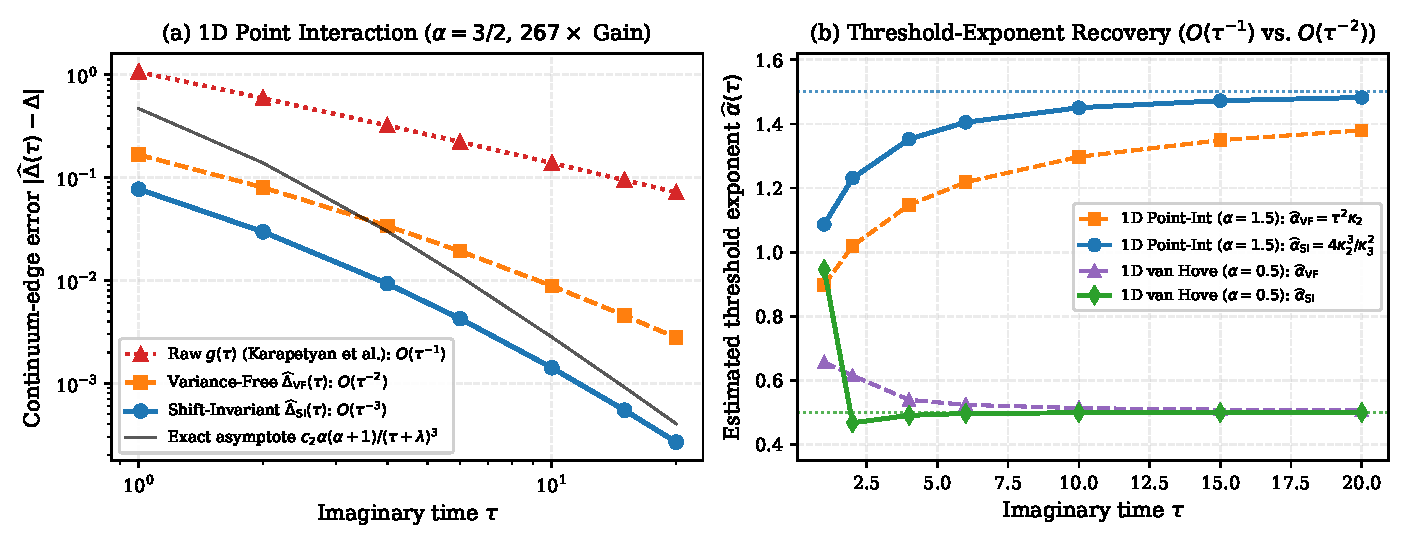
\includegraphics[width=\textwidth]{figures/fig1_shift_invariant_laws.pdf}
  \caption{\textbf{(a)} Continuum-edge gap error $|\widehat{\Delta}(\tau)-\Delta|$ on the 1D point interaction ($\alpha=3/2$, $\Delta=1$), confirming the $O(\tau^{-1})$, $O(\tau^{-2})$, and $O(\tau^{-3})$ scaling laws and exact asymptote $c_2\alpha(\alpha+1)/(\tau+\lambda)^3$ ($267\times$ gain at $\tau=20$). \textbf{(b)} Threshold-exponent recovery $\widehat{\alpha}_{\mathrm{SI}}$ vs.\ $\widehat{\alpha}_{\mathrm{VF}}$ on the 1D point interaction ($\alpha=1.5$) and 1D van Hove band ($\alpha=0.5$).}
  \label{fig:fig1}
\end{figure}

\subsection{Experiment 2: \texorpdfstring{$L=401$}{L=401} Lattice Impurity ED and Spectral-Edge Trichotomy}

To test a discrete finite-lattice Hamiltonian approximating a continuum edge, we exactly diagonalized the 1D tight-binding impurity chain $H = -\sum_{j=0}^{L-2}(|j\rangle\langle j+1|+\mathrm{h.c.}) - V_0 |c\rangle\langle c|$ at $L = 401$, $V_0 = 1.5$ (confirming the bound state $E_0 = -2.500000$ to $10^{-15}$ below the band edge $-2.0$, giving exact thermodynamic gap $\Delta = 0.500000$ and $\alpha = 3/2$ for an initial state at site $c+1$). As shown in Figure~\ref{fig:fig2}(a), at $\tau = 20$, raw $g(20)$ errs by $+0.0733$, whereas $\widehat{\Delta}_{\mathrm{SI}}(20)$ errs by only $+4.33 \times 10^{-4}$ ($\mathbf{169\times}$ gain; reaching $\mathbf{288\times}$ at $\tau = 30$, with $\widehat{\alpha}_{\mathrm{SI}}(30) = 1.4831$ vs.\ $1.50$).

Figure~\ref{fig:fig2}(b) demonstrates Theorem~\ref{thm:trichotomy} across $\tau \in [2, 50]$: for an isolated discrete excited state ($\Delta=1.0, E_2 = 2.5$), $\tau^2\kappa_2(\tau)$ collapses exponentially to $1.00 \times 10^{-29}$ by $\tau = 50$; for power-law continua ($\alpha = 0.5, 1.5$), $\tau^2\kappa_2(\tau)$ converges smoothly to $\alpha$ (with $\widehat{\alpha}_{\mathrm{SI}}(50) = 0.4992, 1.4963$); and for the stretched-exponential pseudogap ($\gamma = 0.5, c = 2.0$), $\tau^2\kappa_2(\tau)$ diverges monotonically as $\Theta(\tau^{1/3})$, reaching $3.28$ at $\tau = 50$.

\begin{figure}[t]
  \centering
  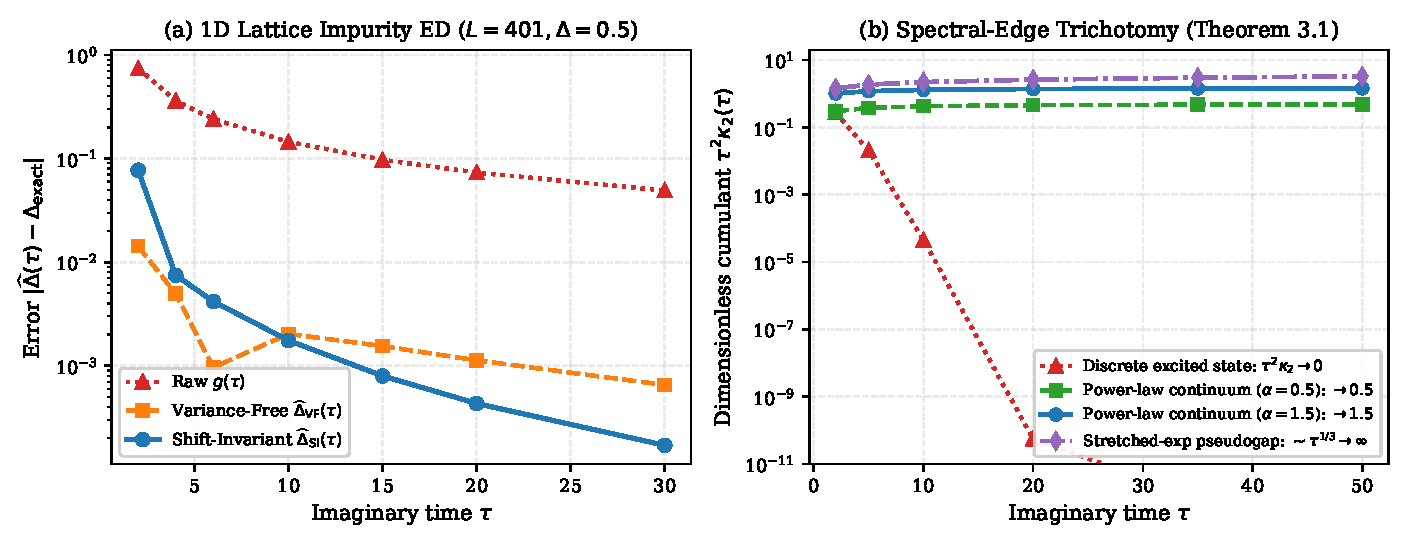
\includegraphics[width=\textwidth]{figures/fig2_lattice_ed_and_trichotomy.pdf}
  \caption{\textbf{(a)} Exact diagonalization of the $L=401$ 1D tight-binding impurity chain ($\Delta=0.5, \alpha=3/2$), showing $169\times$--$288\times$ smaller error from $\widehat{\Delta}_{\mathrm{SI}}$ at $\tau = 20$--$30$. \textbf{(b)} Empirical verification of Theorem~\ref{thm:trichotomy}: $\tau^2\kappa_2(\tau)$ separates discrete excited levels ($\to 0$), power-law continua ($\to \alpha$), and stretched-exponential pseudogaps ($\sim \tau^{1/3} \to \infty$).}
  \label{fig:fig2}
\end{figure}

\subsection{Experiment 3: Exact-\texorpdfstring{$\Q$}{Q} Stieltjes--Hankel Certificates and Noisy Interval Audit}

Using \texttt{build\_exact\_hankel\_certificate} on a fixed small-$\tau$ grid ($\tau_0 = 1.0, \delta = 0.5$), we generated and independently verified 6 zero-float-trust exact-$\Q$ Stieltjes--Hankel upper certificates across all continuum models:
\begin{itemize}[leftmargin=1.6em,itemsep=2pt]
  \item \textbf{Order sweep on 1D point interaction ($\alpha=3/2, \Delta=1.0$, Figure~\ref{fig:fig3}a):} Increasing Hankel order $n = 0 \to 5$ ($\tau_{\max} = 1.5 \to 6.5$) monotonically sharpens the assumption-free exact-$\Q$ upper bound from $\Delta \le 1.8911$ ($n=0$) down to $\mathbf{\Delta \le 1.0879}$ ($n=5$)—$\mathbf{2.35\times}$ tighter than the raw decay rate $g(6.5) = 1.2066$ at the \emph{exact same} maximum horizon $\tau_{\max} = 6.5$, while making zero assumptions on $d\nu$!
  \item \textbf{Cross-model exact-$\Q$ certificates ($n = 4, 5$):} 1D point interaction ($\alpha=1/2$, $\Delta=1.0$) certifies $\Delta \le 1.0239$; 3D point interaction ($\Delta=1.0$) certifies $\Delta \le 1.0806$; 1D van Hove ($\Delta=0.5$) certifies $\Delta \le 0.5255$; 2D step ($\Delta=0.5$) certifies $\Delta \le 0.5502$; and $L=401$ lattice impurity ED ($\Delta=0.5$, $n=4$) certifies $\Delta \le 0.6156$. Every single certificate replays in exact $\Q$ with strictly negative witness margin and verified $\Delta_{\mathrm{ub}}^{\Q} > \Delta_{\mathrm{true}}$.
  \item \textbf{Noisy finite-sample interval soundness:} Across 200 synthetic Gaussian relative-noise trials on the 1D point interaction with Bonferroni enclosures ($z = 3.29$), at $\sigma_{\mathrm{rel}} = 10^{-3}$ ($n=2$) $69\%$ of trials certified with \textbf{200/200 (100\%) soundness} (median $\Delta_{\mathrm{ub}} = 1.669 \ge 1.0$), and at $\sigma_{\mathrm{rel}} = 10^{-2}$ ($n=1$) $97.5\%$ certified with \textbf{200/200 (100\%) soundness} (median $\Delta_{\mathrm{ub}} = 2.573 \ge 1.0$).
\end{itemize}

\begin{figure}[t]
  \centering
  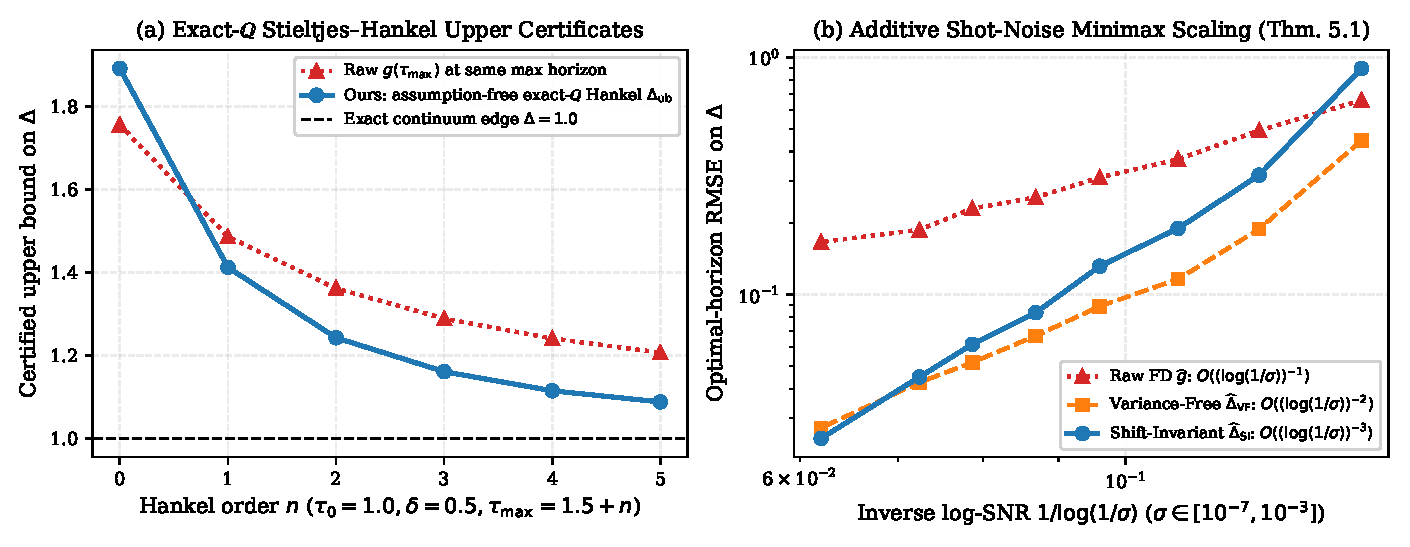
\includegraphics[width=\textwidth]{figures/fig3_hankel_and_minimax.pdf}
  \caption{\textbf{(a)} Assumption-free exact-$\Q$ Stieltjes--Hankel upper certificates $\Delta_{\mathrm{ub}}^{\Q}$ on the 1D point interaction ($\tau_0=1, \delta=0.5$), beating raw $g(\tau_{\max})$ by $2.35\times$ at $n=5$ ($\tau_{\max}=6.5$). \textbf{(b)} Additive shot-noise optimal-horizon RMSE vs.\ $1/\log(1/\sigma)$ ($\sigma \in [10^{-7}, 10^{-3}]$), displaying the $O((\log(1/\sigma))^{-1,-2,-3})$ poly-logarithmic slopes and the honest finite-noise bias--variance crossover between $\widehat{\Delta}_{\mathrm{VF}}$ and $\widehat{\Delta}_{\mathrm{SI}}$.}
  \label{fig:fig3}
\end{figure}

\subsection{Experiment 4: Additive Shot-Noise Minimax Scaling}

Figure~\ref{fig:fig3}(b) tests Theorem~\ref{thm:minimax} directly on the 1D point interaction ($\Delta=1.0, \alpha=3/2$) across 8 additive noise levels $\sigma \in [10^{-7}, 10^{-3}]$ ($120$ Monte Carlo trials each, 5-point stencil $h = 0.50$, with $\tau^*(\sigma)$ oracle-selected over the $\tau$-grid of spacing $0.25$ to trace the theoretical optimal-horizon envelope of Theorem~\ref{thm:minimax}b). As predicted by Theorem~\ref{thm:minimax}(b): (i) raw $\widehat{g}$ stalls at $O(1/\log(1/\sigma))$ (RMSE $0.1662$ even at $\sigma = 10^{-7}$); (ii) at moderate noise ($\sigma \in [10^{-5}, 10^{-3}]$), second-order $\widehat{\Delta}_{\mathrm{VF}}$ achieves the lowest RMSE ($0.0668$ vs.\ $0.2563$ raw at $\sigma = 10^{-5}$, $3.8\times$ better) because $\widehat{\Delta}_{\mathrm{SI}}$ amplifies third-derivative noise; and (iii) as $\sigma$ drops to $10^{-7}$, $\widehat{\Delta}_{\mathrm{SI}}$'s steeper $O((\log(1/\sigma))^{-3})$ slope crosses below $\widehat{\Delta}_{\mathrm{VF}}$, reaching RMSE $\mathbf{0.0247}$ ($\mathbf{6.74\times}$ lower RMSE than raw $\widehat{g}$!).

\section{Discussion, Limitations, and Scope}
\label{sec:discussion}

We have shown that moving from first-order logarithmic decay rates to shift-invariant cumulant combinations ($\widehat{\Delta}_{\mathrm{SI}}, \widehat{\alpha}_{\mathrm{SI}}$) and exact-$\Q$ Stieltjes--Hankel moment certificates eliminates two full orders of finite-$\tau$ bias, cleanly classifies spectral-edge regimes, and provides assumption-free rational upper bounds on continuum spectral edges.

Three honest boundaries frame our results: (i) the $O(\tau^{-3})$ shift-invariant estimator requires estimating the third cumulant $\kappa_3$, which increases sensitivity to additive measurement noise at low SNR (making $\widehat{\Delta}_{\mathrm{VF}}$ preferable at $\sigma \gtrsim 10^{-6}$ and $\widehat{\Delta}_{\mathrm{SI}}$ superior at high SNR or deterministic ITE/tensor-network simulations, as shown in Figure~\ref{fig:fig3}b); (ii) exact-$\Q$ Stieltjes--Hankel witnesses certify \emph{upper} bounds $\Delta < \Delta_{\mathrm{ub}}^{\Q}$ without assumptions, whereas certifying a non-trivial \emph{lower} bound $\Delta > \Delta_{\mathrm{lb}}$ from finite-$\tau$ moments alone is impossible without either an explicit physical structure (such as reflection positivity~\cite{Antigravity2026Purity}) or a known energy-band/moment enclosure~\cite{Antigravity2026QCQMC}, because an arbitrarily tiny spectral weight $10^{-100}\delta_{\Delta'}$ at $\Delta' < \Delta$ can hide inside any finite-precision moment interval; and (iii) on finite-size lattices of size $L$, the discrete level spacing $\delta E \sim \pi^2/L^2$ eventually triggers the discrete regime $\tau^2\kappa_2 \to 0$ once $\tau \gg L^2/\pi^2$, so $\tau$ must remain in the intermediate continuum scaling window $1 \ll \tau \ll L^2/\pi^2$.

\bibliographystyle{plain}
\bibliography{references}

\end{document}
